
\section{Pre-Trained Models}
This section describes the results obtained using different pre-trained architecture and strategies\footnote{The data augmentation strategy is always used since we have very little data}. The pre-trained networks here tested are:
\begin{itemize}
\item VGG16
\item ResNet50V2
\item ResNet101V2
\item InceptionV3
\end{itemize}
 
\subsection{VGG16}
VGG16\ref{fig:vgg16} is a convolutional neural network model proposed by Simonyan et al., with several 3x3 convolutional layers in cascade occasionally interleaved with 2x2 max-pooling layers forming the so called \textit{blocks}. Developed for the ILSVRC2014 challenge, it was able to achieve a top-5 accuracy of 92.7 on ImageNet.
\begin{figure}[H]
	\centering
	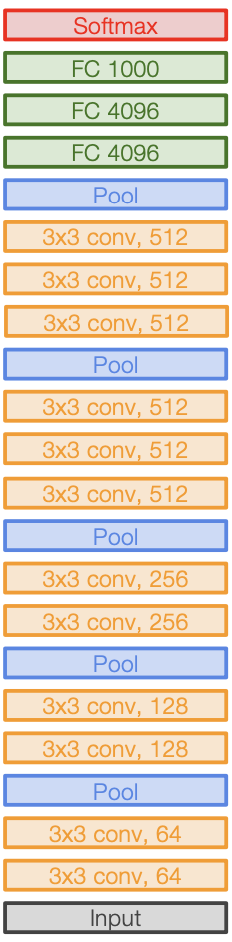
\includegraphics[height=0.7\textwidth]{img/vgg16/vgg16.png}
	\caption{VGG16 Architecture}
	\label{fig:vgg16}
\end{figure}

\subsubsection{Test 1: Classical VGG16 (Feature Extraction)}
The original VGG16 comes with a couple of 4096 FC layers followed by 1000 softmax neurons, which is alright for ImageNet but definitely oversized for our purpose. Hence, the convolutional base is left as it is, and the fully-connected block is replaced by the a shrunk version with only 256 neurons per layer, followed by our prediction layer made of 11 neurons\ref{fig:vgg16fe1}.

\begin{figure}[H]
	\centering
	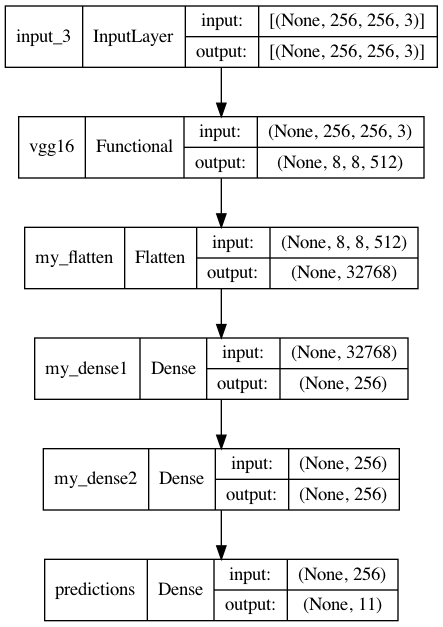
\includegraphics[height=0.5\textwidth]{img/vgg16/vgg16fe1.png}
	\caption{Our Feature Extraction Network}
	\label{fig:vgg16fe1}
\end{figure}


\noindent The result obtained, using RMSprop as optimizer, are:

\medskip

\begin{tabular}{ |p{2cm}|p{2cm}|p{2cm}|p{2cm}|p{2cm}|  }
\hline
\multicolumn{5}{|c|}{Feature Extraction} \\
\hline
\textbf{Epoch stopped} & \textbf{Validation Accuracy} & \textbf{Testing Accuracy} & \textbf{Validation Loss} & \textbf{Testing Loss} \\
\hline
12 & 0.7409 & 0.7057 & 5.1959 & 5.7\\
\hline
\end{tabular}

\medskip

 \noindent The network begin to overfit very fast, hence some regularization methods are needed.


\begin{figure}[H]
	\centering
	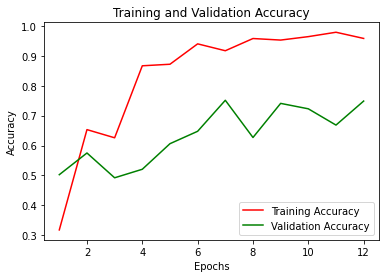
\includegraphics[height=0.45\textwidth]{img/vgg16/vgg16fe1acc.png}
	\caption{Our Feature Extraction Network Accuracy}
	\label{fig:vgg16fe1acc}
\end{figure}

\begin{figure}[H]
	\centering
	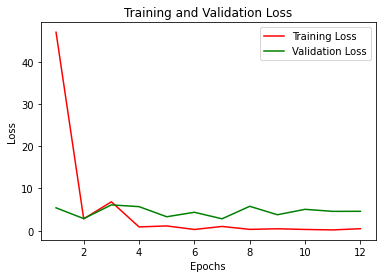
\includegraphics[height=0.45\textwidth]{img/vgg16/vgg16fe1loss.png}
	\caption{Our Feature Extraction Network Loss}
	\label{fig:vgg16fe1loss}
\end{figure}

\subsubsection{Test 2: Adding dropout to Test 1}
We have two possible positions to use the dropout layer in our network and they are after each 256-dense layer, but we decided to use just one layer at the end of the second 256-Dense layer (\textit{my\_dense1}) as shown in Figure\ref{fig:vgg16fe2}. We didn't use a dropout layer between the two 256-dense layers, since this type of architecture led to worst performance, this mainly because we would have less units to fully train our topic-specific network.
\begin{figure}[H]
	\centering
	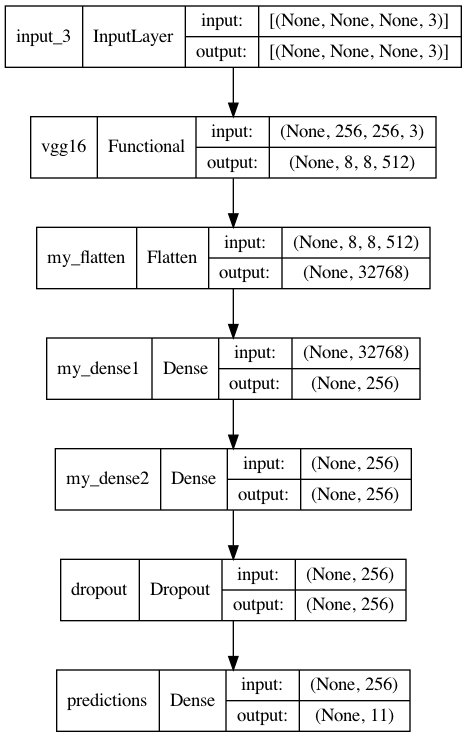
\includegraphics[height=0.45\textwidth]{img/vgg16/vgg16fe2.png}
	\caption{Our Feature Extraction Network + Dropout}
	\label{fig:vgg16fe2}
\end{figure}
  

\noindent The result obtained, using RMSprop as optimizer, are:

\medskip

\begin{tabular}{ |p{2cm}|p{2cm}|p{2cm}|p{2cm}|p{2cm}|  }
\hline
\multicolumn{5}{|c|}{Feature Extraction} \\
\hline
\textbf{Epoch stopped} & \textbf{Validation Accuracy} & \textbf{Testing Accuracy} & \textbf{Validation Loss} & \textbf{Testing Loss} \\
\hline
25 & 0.7306 & 0.7195 & 3.0616 & 3.0035\\
\hline
\end{tabular}

\medskip

\begin{figure}[H]
	\centering
	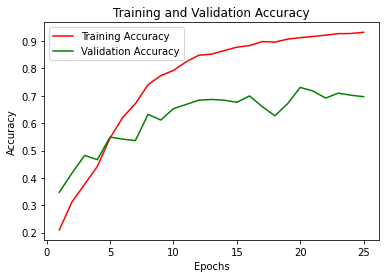
\includegraphics[height=0.45\textwidth]{img/vgg16/vgg16fe2acc.png}
	\caption{Test 2 Accuracy}
	\label{fig:vgg16fe2acc}
\end{figure}

\begin{figure}[H]
	\centering
	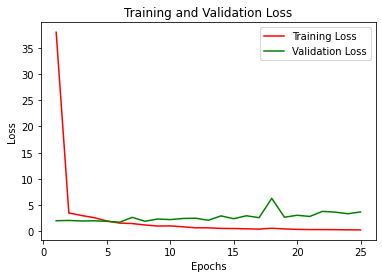
\includegraphics[height=0.45\textwidth]{img/vgg16/vgg16fe2loss.png}
	\caption{Test 2 Loss}
	\label{fig:vgg16fe2oss}
\end{figure}

\noindent TODO: As expected, dropout mitigated the magnitude of overfitting, however our network perform slightly worst (now the validation accuracy is 0.73 and before was 0.74) than without the dropout layer.


\subsubsection{Test 3: Fine Tuning One Convolutional Layer}
Using the model defined in test 1, the 3rd Conv2D layer in the 5th block is un-fronzen and the network is trained. The result obtained using RMSprop as optimizer are the following:

 
 \medskip

\begin{tabular}{ |p{2cm}|p{2cm}|p{2cm}|p{2cm}|p{2cm}|  }
\hline
\multicolumn{5}{|c|}{Feature Extraction} \\
\hline
\textbf{Epoch stopped} & \textbf{Validation Accuracy} & \textbf{Testing Accuracy} & \textbf{Validation Loss} & \textbf{Testing Loss} \\
\hline
28 & 0.7202 & 0.6253 & 2.3687 & 8.1807\\
\hline
\end{tabular}

\medskip

\begin{figure}[H]
	\centering
	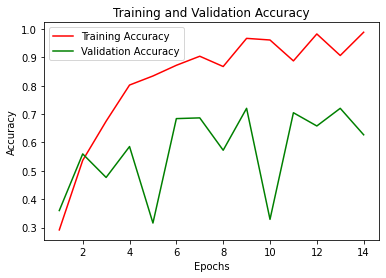
\includegraphics[height=0.45\textwidth]{img/vgg16/vgg16ft1acc.png}
	\caption{Test 3 Accuracy}
	\label{fig:vgg16ft1acc}
\end{figure}

\begin{figure}[H]
	\centering
	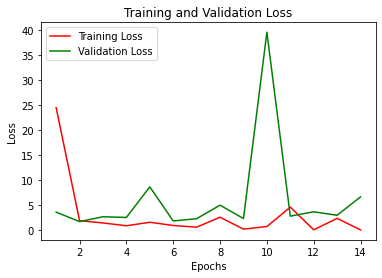
\includegraphics[height=0.45\textwidth]{img/vgg16/vgg16ft1loss.png}
	\caption{Test 3 Loss}
	\label{fig:vgg16ft1loss}
\end{figure}


Again the performance are worst than in test one, but looking at the graphs it can be seen that not only our network overfitted very fast, but it forms also few fang-shaped changes in direction. 






\subsubsection{Test 4: test 3 with dropout and different optimizer}
To overcome the previous problems, the overfitting and the strange shape behavior, in this test we opt to use \textbf{Adam} as an optimizer, changing its default learning rate (i.e., 0.001) to 0.0001 in order to slowly learn and hoping to have a smoother accuracy and loss functions.

 
 \medskip

\begin{tabular}{ |p{2cm}|p{2cm}|p{2cm}|p{2cm}|p{2cm}|  }
\hline
\multicolumn{5}{|c|}{Feature Extraction} \\
\hline
\textbf{Epoch stopped} & \textbf{Validation Accuracy} & \textbf{Testing Accuracy} & \textbf{Validation Loss} & \textbf{Testing Loss} \\
\hline
28 & 0.7358 & 0.7218 & 0.9871 & 1.1792\\
\hline
\end{tabular}

\medskip

\begin{figure}[H]
	\centering
	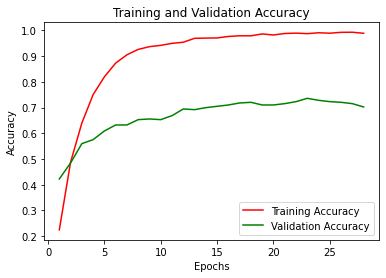
\includegraphics[height=0.45\textwidth]{img/vgg16/vgg16ft1dropacc.png}
	\caption{Test 4 Accuracy}
	\label{fig:vgg16ft1dropacc}
\end{figure}

\begin{figure}[H]
	\centering
	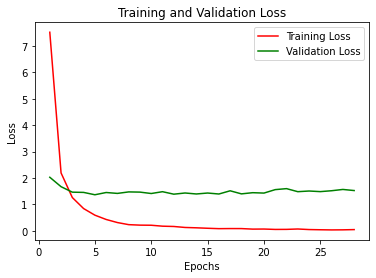
\includegraphics[height=0.45\textwidth]{img/vgg16/vgg16ft1droploss.png}
	\caption{Test 4 Loss}
	\label{fig:vgg16ft1droploss}
\end{figure}

\noindent Adding dropout and a different optimizer with a little learning rate, we finally obtained what we were aiming. Anyway, the result is now comparable to the test 1, however now we our using a more complex network which is not good if the results are the same.

However we can still do something, the training accuracy increases very rapidly even if dropout is applied. To decrease this effect in test 6 we use weight regularization techniques.



\subsubsection{Test 5: Fine Tuning Two Convolutional Layers}
This test is basically test 4, but finetuning the last two convolutional layers of VGG16.

 \medskip

\begin{tabular}{ |p{2cm}|p{2cm}|p{2cm}|p{2cm}|p{2cm}|  }
\hline
\multicolumn{5}{|c|}{Feature Extraction} \\
\hline
\textbf{Epoch stopped} & \textbf{Validation Accuracy} & \textbf{Testing Accuracy} & \textbf{Validation Loss} & \textbf{Testing Loss} \\
\hline
22 & 0.7280 & 0.7379 & 1.4253 & 1.2589\\
\hline
\end{tabular}

\medskip

\begin{figure}[H]
	\centering
	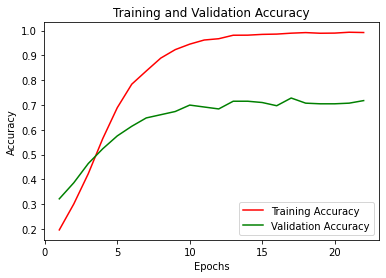
\includegraphics[height=0.45\textwidth]{img/vgg16/vgg16ft2dropacc.png}
	\caption{Test 5 Accuracy}
	\label{fig:vgg16ft2dropacc}
\end{figure}

\begin{figure}[H]
	\centering
	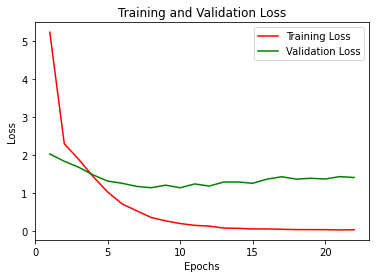
\includegraphics[height=0.45\textwidth]{img/vgg16/vgg16ft2droploss.png}
	\caption{Test 5 Loss}
	\label{fig:vgg16ft2droploss}
\end{figure}

Following the approach used in the previous test we obtained also here more smoothed graphs, but the performance is little lower than before. The problem here is that we are propagating to the second layer in block 5 gradients that are not really improvements of the ones set by the \textit{imagenet} default configuration.






\subsubsection{Test 6: Fine Tuning One Convolutional Layer + weights regularization}
In this paragraph we exploited the conclusion mentioned in test 4, introducing here \textit{L1\_L2 weight regularization} on the one convolutional layer finetuned network.


\medskip

\begin{tabular}{ |p{2cm}|p{2cm}|p{2cm}|p{2cm}|p{2cm}|  }
\hline
\multicolumn{5}{|c|}{Feature Extraction} \\
\hline
\textbf{Epoch stopped} & \textbf{Validation Accuracy} & \textbf{Testing Accuracy} & \textbf{Validation Loss} & \textbf{Testing Loss} \\
\hline
22& 0.7487 & 0.7471 & 21.5590 & 9.8097\\
\hline
\end{tabular}

\medskip

\begin{figure}[H]
	\centering
	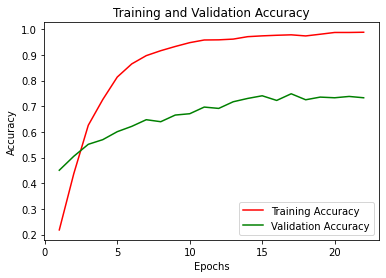
\includegraphics[height=0.45\textwidth]{img/vgg16/vgg16ft1dropregacc.png}
	\caption{Test 6 Accuracy}
	\label{fig:vgg16ft1dropregacc}
\end{figure}

\begin{figure}[H]
	\centering
	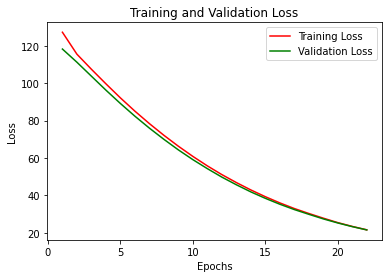
\includegraphics[height=0.45\textwidth]{img/vgg16/vgg16ft1dropregloss.png}
	\caption{Test 6 Loss}
	\label{fig:vgg16ft1dropregloss}
\end{figure}

The shapes of the graphs are more or less the same of the two had in test 4, the only things that changes are the values of the losses which are here higher and more curvilinear due to the weight regularization approach used. Anyway, this heavy regularization helped us to surpass the result in test 1, not by much but it is an improvement that, maybe, can be exploited finetuning more. Following this lead, in the next paragraph we use weight regularization with two convolutional layers finetuned.






\subsubsection{Test 7: Fine Tuning Two Convolutional Layers and Weights Regularization}
Following the good result obtained in test 6, in this paragraph we add, to the network used in test 5, \textit{L1\_L2 weight regularization}.

 \medskip

\begin{tabular}{ |p{2cm}|p{2cm}|p{2cm}|p{2cm}|p{2cm}|  }
\hline
\multicolumn{5}{|c|}{Feature Extraction} \\
\hline
\textbf{Epoch stopped} & \textbf{Validation Accuracy} & \textbf{Testing Accuracy} & \textbf{Validation Loss} & \textbf{Testing Loss} \\
\hline
25 & 0.7694 & 0.7494 & 15.6742 & 9.8097\\
\hline
\end{tabular}

\medskip

\begin{figure}[H]
	\centering
	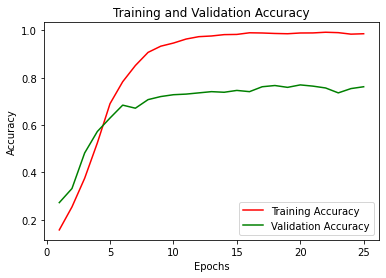
\includegraphics[height=0.45\textwidth]{img/vgg16/vgg16ft2dropregacc.png}
	\caption{Test 7 Accuracy}
	\label{fig:vgg16ft2dropregacc}
\end{figure}

\begin{figure}[H]
	\centering
	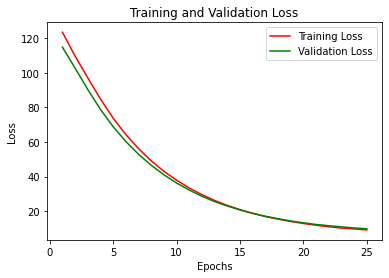
\includegraphics[height=0.45\textwidth]{img/vgg16/vgg16ft2dropregloss.png}
	\caption{Test 7 Loss}
	\label{fig:vgg16ft2dropregloss}
\end{figure}

Even if the increase the flexibility of our network finetuning more layers, as hoped, we achieved a better accuracy which is also the best obtained so far.




\subsubsection{Test 8: Genetic Algorithm for Hyper-parameters and Architecture Optimization}





\subsection{ResNet50V2}


\subsubsection{Test 1: Classical ResNet50V2 (Feature Extraction)}

\begin{tabular}{ |p{2cm}|p{2cm}|p{2cm}|p{2cm}|p{2cm}|  }
\hline
\multicolumn{5}{|c|}{Feature Extraction} \\
\hline
\textbf{Epoch stopped} & \textbf{Validation Accuracy} & \textbf{Testing Accuracy} & \textbf{Validation Loss} & \textbf{Testing Loss} \\
\hline
39 & 0.4430 & 0.3241 & 5.3733 & 6.8513\\
\hline
\end{tabular}

\begin{figure}[H]
	\centering
	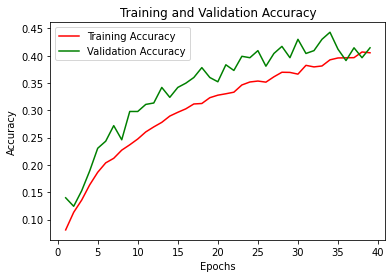
\includegraphics[height=0.45\textwidth]{img/resnet50v2/resnet50acc.png}
	\caption{Our Feature Extraction Network Accuracy}
	\label{fig:resnet50acc}
\end{figure}

\begin{figure}[H]
	\centering
	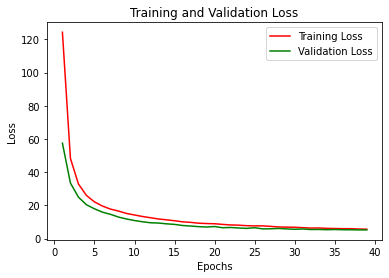
\includegraphics[height=0.45\textwidth]{img/resnet50v2/resnet50loss.png}
	\caption{Our Feature Extraction Network Loss}
	\label{fig:resnet50loss}
\end{figure}


\subsubsection{Test 2: Finetune 1 block}

\begin{tabular}{ |p{2cm}|p{2cm}|p{2cm}|p{2cm}|p{2cm}|  }
\hline
\multicolumn{5}{|c|}{Feature Extraction} \\
\hline
\textbf{Epoch stopped} & \textbf{Validation Accuracy} & \textbf{Testing Accuracy} & \textbf{Validation Loss} & \textbf{Testing Loss} \\
\hline
18 & 0.6399 & 0.5793 & 1.2453 & 1.7916\\
\hline
\end{tabular}

\begin{figure}[H]
	\centering
	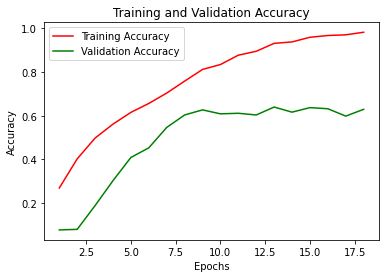
\includegraphics[height=0.45\textwidth]{img/resnet50v2/resnet50finetuned1acc.png}
	\caption{Our Feature Extraction Network Accuracy}
	\label{fig:resnet50finetuned1acc}
\end{figure}

\begin{figure}[H]
	\centering
	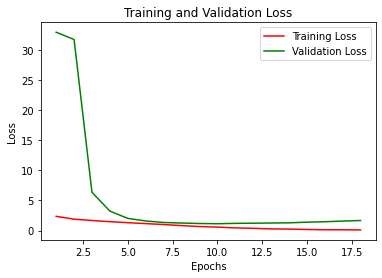
\includegraphics[height=0.45\textwidth]{img/resnet50v2/resnet50finetuned1loss.png}
	\caption{Our Feature Extraction Network Loss}
	\label{fig:resnet50finetuned1loss}
\end{figure}

\subsubsection{Test 3: Finetuned 2 blocks}

\begin{tabular}{ |p{2cm}|p{2cm}|p{2cm}|p{2cm}|p{2cm}|  }
\hline
\multicolumn{5}{|c|}{Feature Extraction} \\
\hline
\textbf{Epoch stopped} & \textbf{Validation Accuracy} & \textbf{Testing Accuracy} & \textbf{Validation Loss} & \textbf{Testing Loss} \\
\hline
20 & 0.6477 & 0.6092 & 1.5918 & 1.7734\\
\hline
\end{tabular}

\begin{figure}[H]
	\centering
	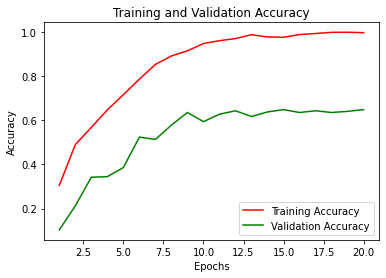
\includegraphics[height=0.45\textwidth]{img/resnet50v2/resnet50finetuned2acc.png}
	\caption{Our Feature Extraction Network Accuracy}
	\label{fig:resnet50finetuned2acc}
\end{figure}

\begin{figure}[H]
	\centering
	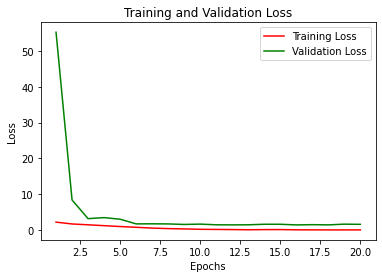
\includegraphics[height=0.45\textwidth]{img/resnet50v2/resnet50finetuned2loss.png}
	\caption{Our Feature Extraction Network Loss}
	\label{fig:resnet50finetuned2loss}
\end{figure}

\subsubsection{Test 4: Fine Tuning with One Layer}

\subsubsection{Test 5: Fine Tuning with Two Layers}







\subsection{ResNet101V2}

\subsubsection{Test 1: Classical ResNet101V2 with 50 classes}

\subsubsection{Test 2: Completely Newly Output Layers Architecture}

\subsubsection{Test 3: Fine Tuning with One Layer}

\subsubsection{Test 4: Fine Tuning with Two Layers}







\subsection{InceptionV3}

\subsubsection{Test 1: Classical ResNet101V2 with 50 classes}

\subsubsection{Test 2: Completely Newly Output Layers Architecture}

\subsubsection{Test 3: Fine Tuning with One Layer}

\subsubsection{Test 4: Fine Tuning with Two Layers}


